\section{Konfiguration eines Skills} \label{Skillkonfiguration}
	Nicht jeder Skill benötigt alle Zustände. Damit der Skill so übersichtlich wie möglich bleibt, sollen auch nur die Zustände verwendet werden, welche benötigt werden. Ein Skill kann drei Konfigurationen einnehmen (Abb. \ref{fig:Skillkonfiguration}).
	\\
	\begin{figure}[h!]
		\centering
		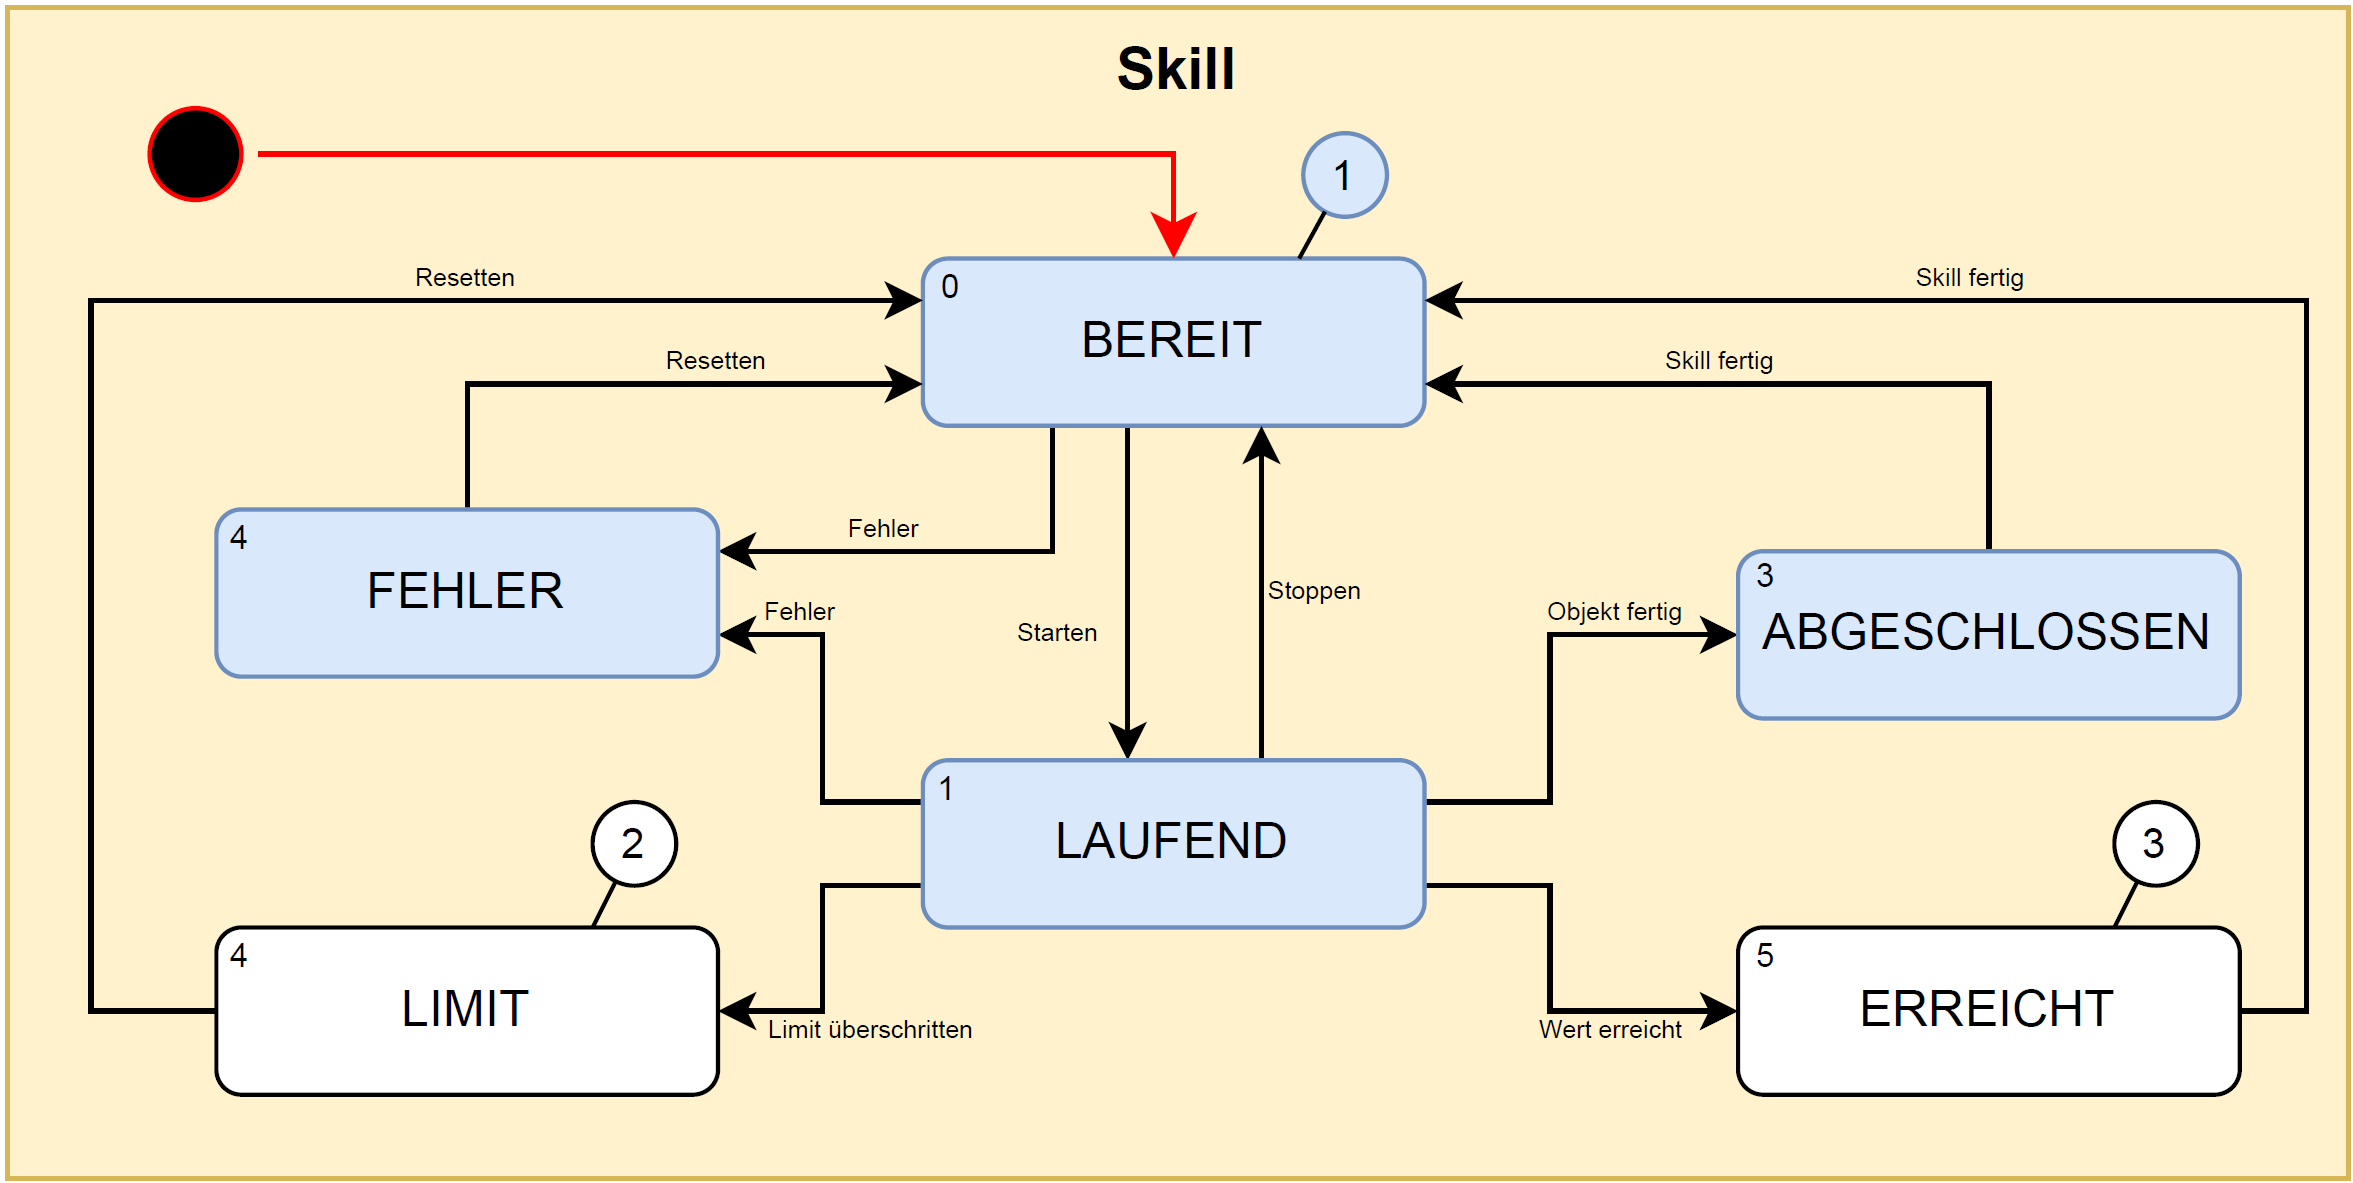
\includegraphics[width=0.8\textwidth]{06_Skillentwicklung/Skillkonfiguration}
		\captionsetup{justification=centering}
		\caption{Skillkonfiguration}
		\label{fig:Skillkonfiguration}
	\end{figure}
	
	\begin{tabularx}{\textwidth}{@{}>{}p{8em} X@{}}
		Konfiguration 1: & 
		Stellt die Grundkonfiguration dar. Jeder Skill muss diese Zustände implementieren. Hierbei handelt es sich um Skills, welche nur durch das Objekt abgeschlossen werden, z.B. eine einfache Punkt-Zu-Punkt-Bewegung des Roboters.
		\\
		Konfiguration 2: & 
		Bei dieser Konfiguration kommt der \verb|LIMIT|-Zustand dazu. Dieser wird benötigt, wenn es eine Limit-Bedingung gibt, z.B. einen Grenzwert für die Kraft oder eine maximale Zeitdauer.
		\\
		Konfiguration 3: & 
		Bei der letzten Konfiguration wird der \verb|ERREICHT|-Zustand ergänzt. Dieser gibt an, ob ein definiertes Ziel erreicht wurde, dies kann z.B. eine Kraft sein.
		\\
	\end{tabularx}